% chktex-file 1
% chktex-file 26
% chktex-file 44
\documentclass{article}
% chktex-file 34
% chktex-file 18
% chktex-file 1
\usepackage{amsfonts}
\usepackage[T1]{fontenc}
\usepackage{amsmath}
\usepackage{amssymb}
\usepackage{mathrsfs}
\usepackage{extarrows}
\usepackage{hyperref}
\usepackage[utf8]{inputenc}
\usepackage{graphicx}
\usepackage{mathtools}
\usepackage[a4paper, total={6in, 8in}]{geometry}
\usepackage[table]{xcolor}
\usepackage{tikz}
\usepackage{cancel}
\usepackage{steinmetz}
\usepackage{diagbox}
\usepackage{siunitx}
\usepackage{eurosym}
\usepackage{pgfplots}
\pgfplotsset{width=10cm,compat=1.9}
\usetikzlibrary{shapes,arrows}
\usepackage{listings}
\usepackage{color}
%definizione colori per blocchi di codice
\definecolor{lightgray}{rgb}{.95,.95,.95}
\definecolor{darkgray}{rgb}{.4,.4,.4}
\definecolor{purple}{rgb}{0.65, 0.12, 0.82}
\definecolor{ocherCode}{rgb}{1, 0.5, 0}
\definecolor{blueCode}{rgb}{0, 0, 0.93}
\definecolor{greenCode}{rgb}{0, 0.6, 0}

%formattazione per i blocchi di codice
\lstset{
  %Special characters
  literate={á}{{\'a}}1 {é}{{\'e}}1 {í}{{\'\i}}1 {ó}{{\'o}}1 {ú}{{\'u}}1 {Á}{{\'A}}1 {É}{{\'E}}1 {Í}{{\'I}}1 {Ó}{{\'O}}1 {Ú}{{\'U}}1 {à}{{\`a}}1 {è}{{\`e}}1 {ì}{{\`\i}}1 {ò}{{\`o}}1 {ù}{{\`u}}1 {À}{{\`A}}1 {È}{{\`E}}1 {Ì}{{\`I}}1 {Ò}{{\`O}}1 {Ù}{{\`U}}1 {ä}{{\"a}}1 {ë}{{\"e}}1 {ï}{{\"\i}}1 {ö}{{\"o}}1 {ü}{{\"u}}1 {Ä}{{\"A}}1 {Ë}{{\"E}}1 {Ï}{{\"I}}1 {Ö}{{\"O}}1 {Ü}{{\"U}}1 {â}{{\^a}}1 {ê}{{\^e}}1 {î}{{\^\i}}1 {ô}{{\^o}}1 {û}{{\^u}}1 {Â}{{\^A}}1 {Ê}{{\^E}}1 {Î}{{\^I}}1 {Ô}{{\^O}}1 {Û}{{\^U}}1 {ã}{{\~a}}1 {ẽ}{{\~e}}1 {ĩ}{{\~\i}}1 {õ}{{\~o}}1 {ũ}{{\~u}}1 {Ã}{{\~A}}1 {Ẽ}{{\~E}}1 {Ĩ}{{\~I}}1 {Õ}{{\~O}}1 {Ũ}{{\~U}}1 {œ}{{\oe}}1 {Œ}{{\OE}}1 {æ}{{\ae}}1 {Æ}{{\AE}}1 {ß}{{\ss}}1 {ű}{{\H{u}}}1 {Ű}{{\H{U}}}1 {ő}{{\H{o}}}1 {Ő}{{\H{O}}}1 {ç}{{\c c}}1 {Ç}{{\c C}}1 {ø}{{\o}}1 {Ø}{{\O}}1 {å}{{\r a}}1 {Å}{{\r A}}1 {€}{{\euro}}1 {£}{{\pounds}}1 {«}{{\guillemotleft}}1 {»}{{\guillemotright}}1 {ñ}{{\~n}}1 {Ñ}{{\~N}}1 {¿}{{?`}}1 {¡}{{!`}}1 {'"'}{\textquotesingle "\textquotesingle}3,
  %Basic design
  backgroundcolor=\color{lightgray},
  frame=l,
  % Line numbers
  xleftmargin={0.75cm},
  numbers=left,
  numberstyle=\footnotesize,
  numbersep=9pt,
  stepnumber=1,
  firstnumber=1,
  numberfirstline=true,
  % Code design
  identifierstyle=\color{black},
  keywordstyle=\color{blue}\bfseries,
  ndkeywordstyle=\color{ocherCode}\bfseries,
  stringstyle=\color{greenCode}\ttfamily,
  commentstyle=\color{darkgray}\ttfamily,
  %Code
  columns=[c]fixed,
  extendedchars=true,
  upquote=true,
  breaklines=true,
  showstringspaces=false,
  showspaces=false,
  tabsize=2,
  breaklines=true,
  showtabs=false,
  captionpos=b
}
%lingue supportate:
%ABAP
%ACSL
%Ada
%Algol
%Ant
%Assembler
%Awk
%bash
%Basic
%C#5
%C++
%C
%Caml
%Clean
%Cobol
%Comal
%csh
%Delphi
%Eiffel
%Elan
%erlang
%Euphoria
%Fortran
%GCL
%Go (golang)
%Gnuplot
%Haskell
%HTML
%IDL
%inform
%Java
%JVMIS
%ksh
%Lisp
%Logo
%Lua
%make
%Mathematica
%Matlab
%Mercury
%MetaPost
%Miranda
%Mizar
%ML
%Modelica
%Modula-2
%MuPAD
%NASTRAN
%Oberon-2
%Objective C
%OCL
%Octave
%Oz
%Pascal
%Perl
%PHP
%PL/I
%Plasm
%POV
%Prolog
%Promela
%Python
%R
%Reduce
%Rexx
%RSL
%Ruby
%S4
%SAS
%Scilab
%sh
%SHELXL
%Simula
%SQL
%tcl4
%TeX
%VBScript
%Verilog
%VHDL
%VRML
%XML
%XSLT

\newcommand{\acapo}{\\\hspace*{1cm}\\}
\newcommand{\Eaccentata}{$\grave{\text{E}}$ }
\newcommand{\vopen}{``}
\newcommand{\apexopen}{`}
\newcommand{\vclose}{''}
\newcommand{\vclosespace}{'' }
\newcommand{\indenta}{\hspace*{1cm}}
\newcommand{\define}{\underline{Def:} }

\setlength{\parindent}{0cm}

\hfuzz=100pt

\author{Flavio Colacicchi}

\title{Prima iterazione\\\normalsize Analisi e progettazione del software}
\date{13/03/2025}
\begin{document}
\maketitle
L'analisi enfatizza un'investigazione di un problema e dei suoi requisiti, ovvero si focalizza sul che cosa e non sul come, e non è direttamente interessata alle soluzioni del problema.\acapo
Esistono diversi modi per effettuare l'analisiciascuno dei quali è in qualche modo legato a una “strategia risolutiva” che si vuole adottare o a uno specifico “tipo di sistema” che si vuole realizzare\acapo
L'analisi orientata agli oggetti (OOA) si basa principalmente sull'identificazione dei concetti nel dominio del problema e su una loro descrizione a oggetti\acapo
L'analisi del software ha lo scopo di comprendere il problema e si deve focalizzare su tre aspetti
\begin{enumerate}
    \item Le inormazioni che il sistema deve gestire (dominio informativo)\\
        Rappresentato attraverso il modello di dominio
    \item Le funzioni (o operazioni) che il sistema dovrà gestire (alterazioni al dominio informativo)\\
        Rappresentate con operazioni di sistema e diagrammi di sequenza di sistema
    \item Il comportamento del sistema (come cambia la rappresentazione del sistema a seguito di operazioni)\\
        Rappresentato tramite contratti
\end{enumerate}
Lo scopo della modellazione è comprendere e favorire la comunicazione.\acapo
Il dominio del problema è simile alla progettazione concettuale delle basi di dati:
\begin{itemize}
    \item Rappresentare le specifiche formali della realtà di interesse
    \item In termini di una descrizione formale e compatta
    \item Indipendente dai scriteri di rappresentazione utilizzati nei sistemi di gestione
\end{itemize}
Mentre nella modellazione del dominio
\begin{itemize}
    \item 
\end{itemize}
\begin{center}
    \begin{tabular}{p{0.5\textwidth}|p{0.5\textwidth}}
        basi di dati & ingegneria del software\\
        \hline
        i diagrammi si chiamano schemi & i diagrammi si chiamano modelli\\
        formalismi per esprimere schemi si chiamano modelli (e.g. Schemi E.R.) & i formalismi per esprimere i modelli si chiamano linguaggi (e.g. UML)
    \end{tabular}
    \begin{tabular}{p{0.5\textwidth}|p{0.5\textwidth}}
        ER & UML\\
        \hline
        Un'entità rappresenta una classe di oggetti che hanno proprietà comune & una classe concettuale
        rappresenta un insieme di
        cose o concetti con
        caratteristiche simili\\
        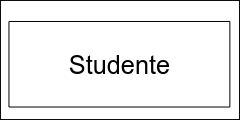
\includegraphics[width=3cm]{images/er.png} & 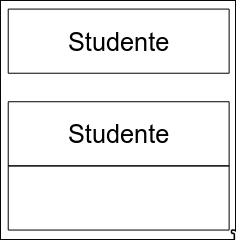
\includegraphics[width=3cm]{images/uml.png}\\
        le relative istanze sono chiamate istanze o occorrenze & le relative istanze sono chiamate istanze o oggetti\\
        un attributo descrive una proprietà elementare di un'entità o di una relazione & un attributo rappresenta una proprietà elementare degli oggetti di una classe\\
        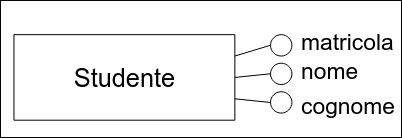
\includegraphics[width=3cm]{images/er2.png} & 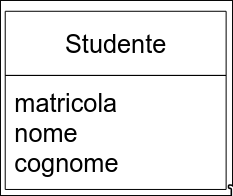
\includegraphics[width=3cm]{images/uml2.png}\\
        una relazione rappresenta un legame logico tra due o più entità & un'associazione rappresenta una relazione (una connessione significativa) tra classi e le istanze si chiamano collegamenti\\
        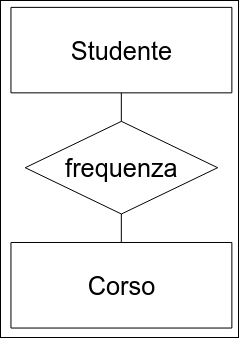
\includegraphics[width=3cm]{images/er3.png} & 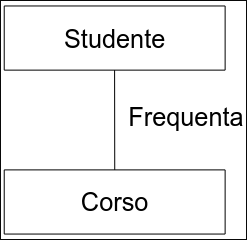
\includegraphics[width=3cm]{images/uml3.png}
    \end{tabular}
    \begin{tabular}{p{0.5\textwidth}|p{0.5\textwidth}}
        le relazioni possono essere binarie o anche N-arie & le associazioni sono in genere binarie e le associazioni N-arie sono possibili, ma poco comuni\\
        Le relazioni possono avere attributi & è possibile rappresentare associazioni con attributi, ma è poco comune\\
        il nome è generalmente un sostantivo che indica una relazione & il nome è generalmente un verbo che indica una relazione\\
        per ciascuna entità va indicato (almeno) un identificatore & è possibile associare identificatori alle classi, ma è poco comune\\
        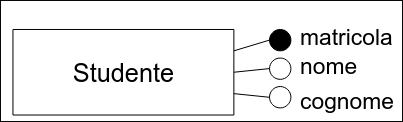
\includegraphics[width=4cm]{images/er4.png} & 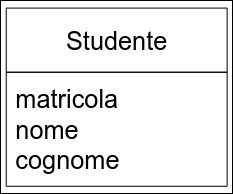
\includegraphics[width=3cm]{images/uml4.png}\\
        una cardinalità caratterizza la partecipazione (minima e massima) di un'entità a una relazione & una molteplicità indica quante istanze di una classe possono essere associate a un'istanza dell'altra classe\\
        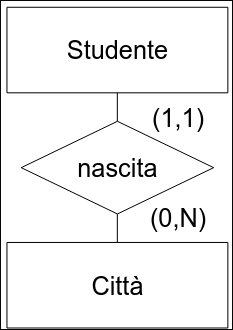
\includegraphics[width=4cm]{images/er5.png} & 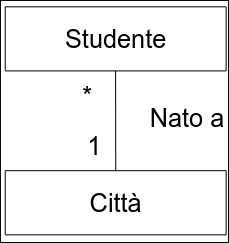
\includegraphics[width=3cm]{images/uml5.png}
    \end{tabular}
    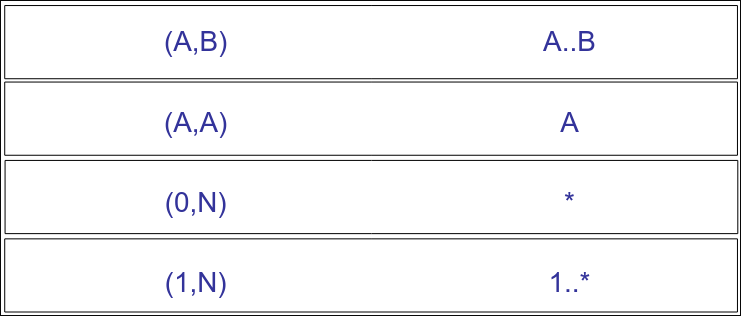
\includegraphics[width=\textwidth]{images/er-uml.png}
    \begin{tabular}{p{0.5\textwidth}|p{0.5\textwidth}}
        per rappresentare solo informazioni che devono essere gestite in modo persistente & per rappresentare tutte le informazioni che devono essere gestite da un'applicazione\\
        un'entità rappresenta sia una classe di istanze che il relativo \vopen insieme\vclose & una classe rappresenta una classe di oggetti ma non il relativo \vopen insieme\vclose\\
        in genere nessuna entità ha una sola istanza & può essere ok avere classi che hanno un solo oggetto\\
        le entità hanno in genere almeno un attributo & può essere ok avere classi senza attributi con cautela\\
        le entità rappresentano informazioni & può essere ok avere classi che rappresentano solo comportamento con cautela
    \end{tabular}
\end{center}
Esempio di rappresnetazione tramite UML di un dominio
\begin{center}
    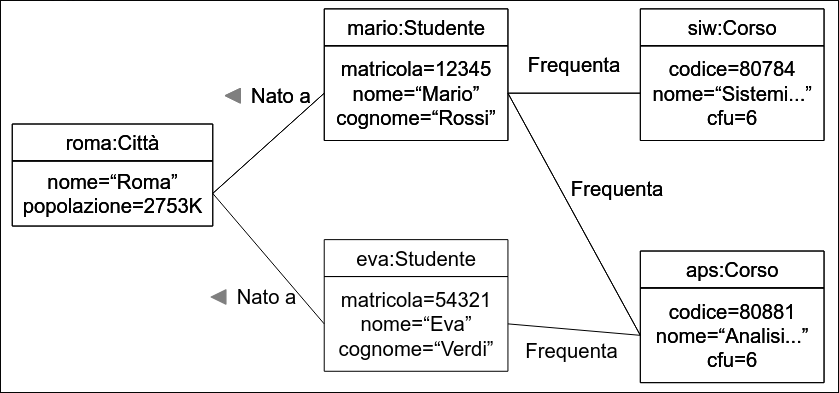
\includegraphics[width=\textwidth]{images/esempio dominio di informazione.png}
\end{center}
Notare che i \textbf{:} sono \textbf{obbligatori per la definizione di un oggetto} mentre sono \textbf{vietati denna definizione di una classe}
\end{document}